\section{Auswertung}
\label{sec:Auswertung}

\subsection{Kontrast}
Zunächst wird der Kontrast berechnet.
Die entsprechenden Messwerte finden sich in \autoref{tab:kontrast}.
Nun lässt sich mit \autoref{eq:kontrast} der Kontrast berechnen. 
Dabei wird die Intensität gleichgesetzt mit der Spannung.
Die Ergebnisse finden sich in der rechten Spalte von \autoref{tab:kontrast}.
\input{build/kontrast.txt}
Als Fit wird die Funktion 
\begin{equation*}
    f(x) = A \cdot \sin(2 x - \delta)
\end{equation*}
angenommen. Dies ist wegen der Proportionalität aus \autoref{eq:kontrast2} gerechtfertigt.
\begin{figure}
    \centering
    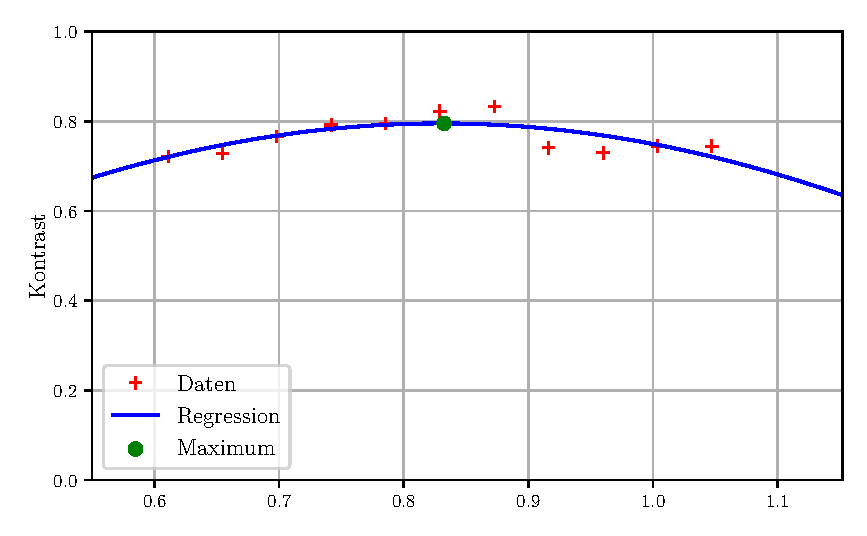
\includegraphics[width = 0.7 \linewidth]{build/Kontrast.pdf}
    \caption{Fit der Theoriekurve an die Messdaten.}
    \label{fig:plot1}
\end{figure}
Der Fit ist in \autoref{fig:plot1} zu sehen.
Für die Variablen ergibt sich $\delta = 0.0877 \pm 0.038$ und $A = 0.8 \pm 0.0085$.
Hieraus ergibt sich das theoretische Maximum von $K = 0.8$ bei einem Winkel von $47.69°$.

\subsection{Brechungsindex Glas}
Nun wird der Brechungsindex von Glas bei einer Rotation von $11°$ und einer Dicke von $T = 1 \unit{\milli\meter}$ berechnet.
Die Messdaten sind in \autoref{tab:glas} zu finden.
Mithilfe von Formel \autoref{eq:nluft} lässt sich nun der Brechungsindex bestimmen.
Auch diese Ergebnisse sind in \autoref{tab:glas} zu finden.
\input{build/n_glas.txt}

% \subsection{Brechungsindex Luft}
% \begin{figure}
%     \centering
%     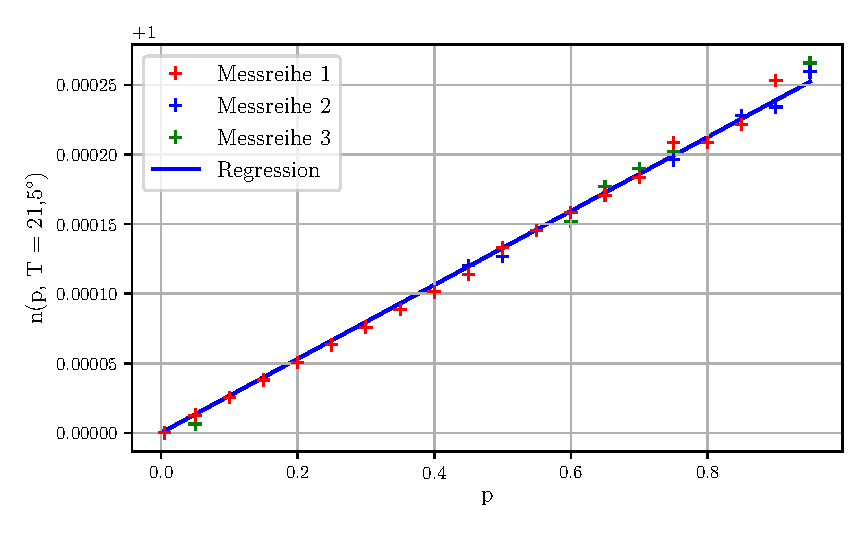
\includegraphics[width = 0.7 \linewidth]{build/Luft.pdf}
%     \caption{Lineare Regression an die Maxima.}
%     \label{fig:plot2}
% \end{figure}
% Die Messdaten der drei Messreihen sind in \autoref{tab:luft} zu finden.
% Zum Zeitpunkt der Messung betrug der Atmosphärendruck $950 \unit{\milli\bar}$ und die Raumtemperatur $T = 21.5 \unit\degree$.
% \input{build/n_luft.txt}
% Nun wird ein Fit an die Maxima angesetzt.
% Dabei wird von einem linearen Zusammenhang ausgegangen, also
% \begin{equation*}
%     M(p) = a + p \cdot m \, .
% \end{equation*}
% Der entsprechende Plot ist in \autoref{fig:plot2} zu sehen.
% Daraus ergibt sich dann für die Variablen $a = -0.68 \pm 0.17$ und $43.02 \pm 0.31$.
% Als beste Schätzung der Maxima bis Atmosphärendruck ergibt sich $M = 40.2 \pm 0.34$, woraus sich mit \autoref{eq:nluft2} der Brechungsindex für Luft zu
% \begin{equation}
%     n_\text{Luft} = 1.0001338 \pm 0.0000011
% \end{equation}
% berechnen lässt.


\subsection{Brechungsindex Luft}
\begin{figure}
    \centering
    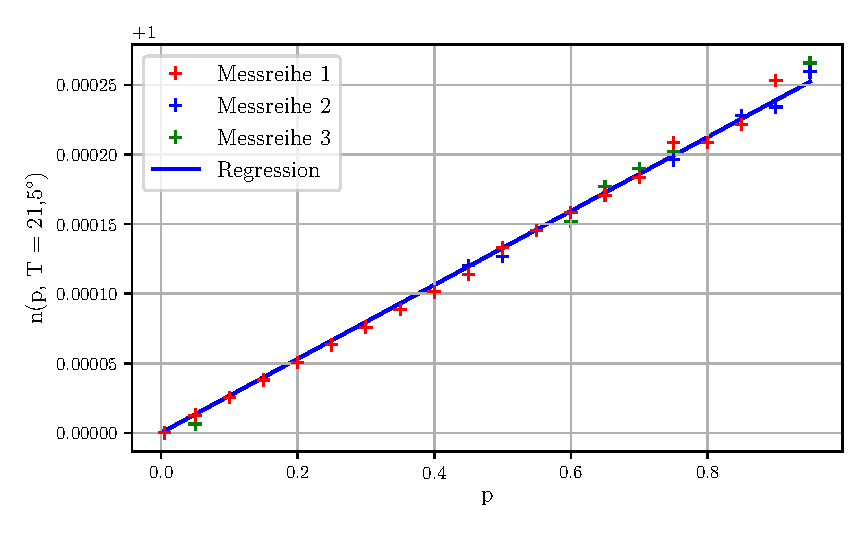
\includegraphics[width = 0.7 \linewidth]{build/Luft.pdf}
    \caption{Lineare Regression an die Brechungsindizes.}
    \label{fig:plot2}
\end{figure}
Die Messdaten der drei Messreihen sind in \autoref{tab:luft} zu finden.
Zum Zeitpunkt der Messung betrug der Atmosphärendruck $950 \unit{\milli\bar}$ und die Raumtemperatur $T = 21.5 \unit\degree$.
\input{build/n_luft.txt}
\input{build/n_berechnet_tabelle.txt}
Aus den Maxima wird nun mithilfe \autoref{eq:nluft2} der dazugehörige Brechungsindex berechnet.
Diese sind in \autoref{tab:n_berechnet} eingetragen und außerdem in \autoref{fig:plot2} aufgetragen.
Nun wird mithilfe des Lorentz-Lorenz-Gesetzes, siehe \autoref{eq:lorentz}, ein Fit durchgeführt.
Das Gesetz wird durch die Funktion
\begin{equation} \label{eq:lorentz2}
    n(p) = 1 + \frac{p \cdot m}{T}
\end{equation}
an die berechneten Brechungsindizes gefittet. Dabei wird für T zunächst $21.5\unit{\celsius}$ eingesetzt.
Es ergibt sich der Plot in \autoref{fig:plot2}.
Der Fit ergibt für $m = 0.07825 \pm 0.00034$.
Nun lässt sich mithilfe von \autoref{eq:lorentz2} der Brechungsindex bei Normalbedingungen ($T = 15 \unit{\celsius}$, $p = 1,013 \unit{\bar}$) zu $n_{\text{norm}} = 1.0002751 \pm 0.0000012$ berechnen.